\subsubsection{Prophet} \label{sec:design-prophet}

Since OlaVM uses a reduced instruction set, some complex computations can only be supported by other means.The most
traditional way is to implement it with existing instructions, but this may take up many opcodes, and there is an upper
limit to the size of Trace, so only if each opcode takes up small enough trace cells, the whole Trace can accommodate more
computations;you can also refer to the design of EVM, and for complex computations, you can support it as a pre-compiled
contract.In this mode, it is not necessary to use EVM instructions to implement this complex computation, but only need
to add the corresponding pre-compile contract, which can be implemented in any high-level language, such as rust, go, etc.
However, this approach will significantly increase the proof workload, and a separate trace table for this complex computation,
and then perform the constraint proof, in the CPU trace, only the output of this computation and the output will be recorded.

\begin{figure}[!ht]
    \centering
    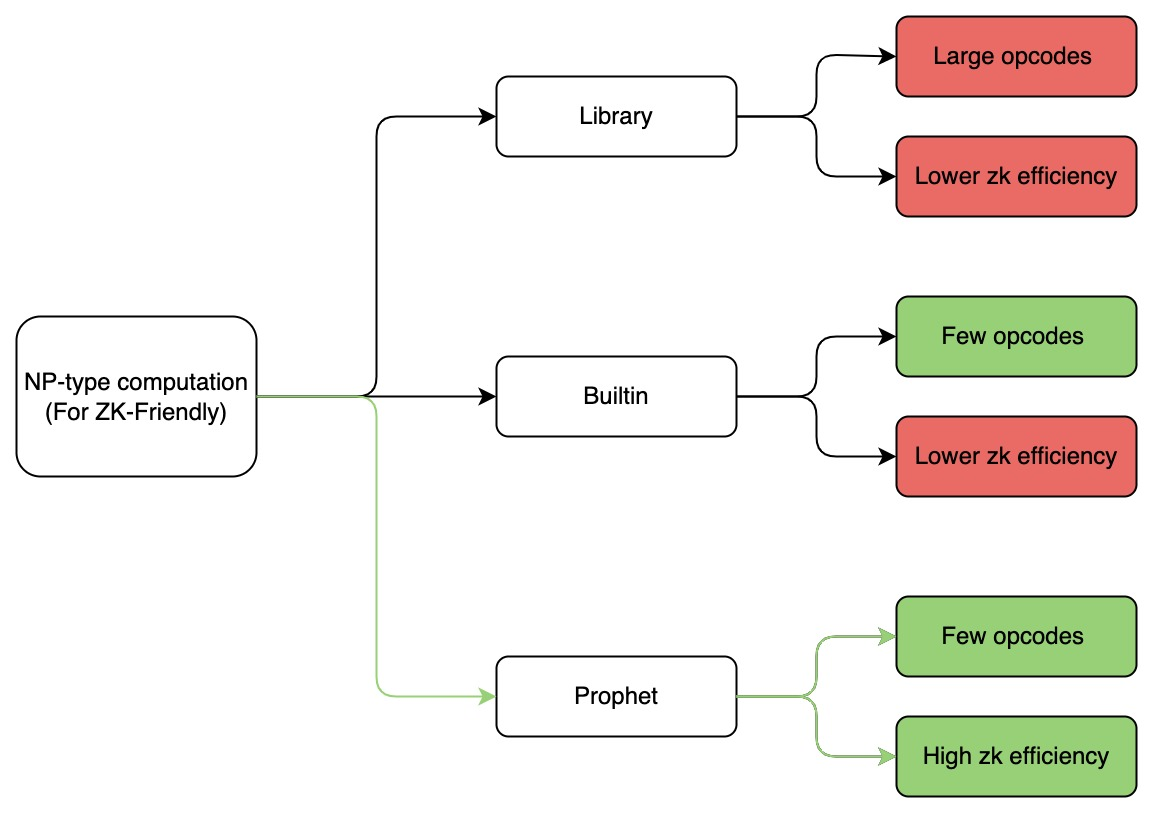
\includegraphics[width=0.5\textwidth]{vm/design-prophet.jpeg}
    \caption{How the Prophet can get ZK-Friendly}
    \label{fig:design-prophet}
\end{figure}

It is desirable to have a method that can support complex computations with few opcodes without significantly increasing the
complexity of the proof;in OlaVM, we call this scheme Prophet, which is shown in\ref{fig:design-prophet}, from the perspective
of prophecy followed by confirmation.From the point of view of prophecy and then confirmation, it fits well with its position
in the overall design.For complex computations, the result of the complex computation is first computed locally by someone else
(often Prover himself), without being constrained during this local computation, and then the VM performs a validity check on the
result before proceeding with the rest of the computation.This verification process is implemented by instructions and is therefore
included in the proof process.

For example: calculate the square root of a radicand.To implement Newton's method need more then 20 instructions, but by contrast,
verify a result is the square root of a radicand is succinct.ZKVM only need to use the result multiply itself to get a product, 
and verify if the product is equal to the radicand.Only use two instructions.By the second algorithm, how to compute the square
root is no matter to ZK circuit and user.The process of computation is wrapped up in prophet segment and not need to be verified
by ZK circuit.ZK circuit only need to verify the succinct logic $\texttt{result} \cdot \texttt{result} == \texttt{radicand}$.
Use OlaVM to execute two algorithm and generate ZK proof, The second algorithm is 10 times faster than the first traditional algorithm.
reference: \ref{subsec: prophet-interpreter}

To ensure that it is developer-friendly at the language level, OlaVM does not support developers to write Prophet themselves for
the time being.The Prophet library is officially maintained and updated for the time being, and to ensure security, the access to
memory during Prophet execution is read-only memory.

It is worth noting that not all complex calculations are suitable for this model, the kind of calculations that are complex to implement
and efficient to verify are more suitable for this approach, common ones such as square root, cube root, etc.; there are also some calculations
that are not complex but still ZK-Unfriendly, such as Bitwise, Rangecheck, Hash and other calculations.These calculations are not suitable
for Prophet's design;we will use the pre-compiled way to support, which is consistent with the pre-compiled contract function in EVM, we
call this way Builtin, in the subsequent chapters, we will introduce the type of Builtin and the way of constraint in detail.